%\newpage
\section{Resistor Measurement}
Each resistor is measured with four different types of measurement in one current direction.
The same resistor ist also tested with the same four measurement types in the other current direction.
The measurement in the opposite direction is only used to identify a resistor.
If mismatch between both measurements is too big, it's not a resistor.

\subsection{Resistor Measurement with 680 Ohm Resistors}
The measurement of a unknown resistor Rx is done in two ways with the build in precision
 \(680\Omega\) resistors. The diagram of this measurements for test pin 1 (TP1) and test pin 3 (TP3) are
 simplified shown in figure~\ref{fig:RL1mes} and figure~\ref{fig:RL2mes} as a example of the six choises of probe combinations.

\begin{figure}[H]
\centering
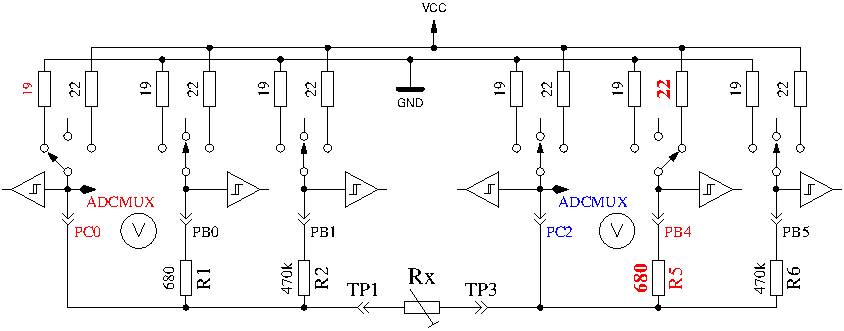
\includegraphics[width=.8\textwidth]{../FIG/ResistormessL1.pdf}
\caption{Measurement type 1 with \(680\Omega\) }
\label{fig:RL1mes}
\end{figure}

\begin{figure}[H]
 \centering
 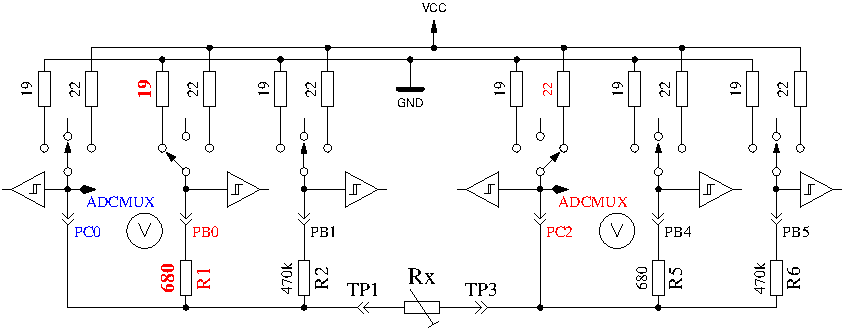
\includegraphics[width=.8\textwidth]{../FIG/ResistormessL2.pdf}
 \caption{Measurement type 2 with \(680\Omega\) }
\label{fig:RL2mes}
\end{figure}

On the left side test pin 1 is shown and on the right side you can see test pin 3.
In both diagrams you see, that the terminal 3 (right side) is connected to VCC, the left side is
connected to GND. The direction of current flow through the resistor Rx is allways the same. 
The values of ports switched to output are shown with red color, the values of 
ports used as Input are shown in blue color, the inactive ports are black.
In both shown measurement types the current should have the same value, because the sum of resistor values
between VCC and GND is identical (if the build in resistors are identical).
Usually the measured voltage is not the same, because the sequence
of resistors has changed.

The V symbol within the circle marks the ports used for voltage measurement.
In both configurations the value of resistor Rx can be computed with the known
resistor values and the measured voltages, if the relation of resistor Rx and the \(680\Omega\) is not too high.
The theoretical voltage gradient is shown in figure~\ref{fig:RLvtot}, where resistor values are shown in logarithmic scale.
\begin{figure}[H]
\centering
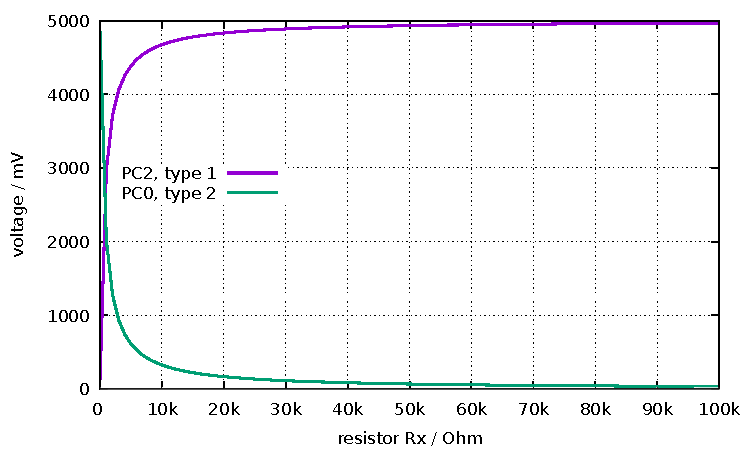
\includegraphics[width=.93\textwidth]{../GNU/RLvtot.pdf}
\caption{Voltages of type 1 and type 2 measurements with \(680\Omega\) }
\label{fig:RLvtot}
\end{figure}
The graph of measurement type 1 is shown in figure~\ref{fig:RLvlow} with zoomed scale for the lower resistor range.
You can see, that you need a better ADC resolution than the standard \(4.9mV\) resolution at the \(5V\) ADC reference, to get
the right resistor value from measured voltage below \(2\Omega\).
There are only three ADC steps from \(0\Omega\) to \(2\Omega\).
The range switching with the AUTOSCALE\_ADC option can help in this case.
The same zoomed range of measurement type 2 shows the figure~\ref{fig:RLvhigh}.
Unfortunately we can not use the higher ADC resolution for measurement type~2 in this range,
 because the voltage is too high and our ATmega have no differential ADC input.
Measurements with the \(680\Omega\) resistors are taken for building the result of measurements up to \(20k\Omega\)
(Voltage of measurement type 2 will be below \(169mV\)).

For higher resistor values the measurements with the \(470k\Omega\) resistors are used. The mean value of both
measurements is taken as displayed resistor value, if all tests attests, that it is no other type of part.
If the AUTOSCALE\_ADC function is selected and one of the voltages of the both measurement types is below \(0.98V\),
a weighted average is build with factor four for this value. The other value is weighted with factor one.
This is done to respect the factor four better resolution of this measurement. Factor four is only taken for 
ATmega168 and ATmega328 processors, for the ATmega8 two is taken as weighting factor if voltage is below \(0.98V\),
because the reference voltage for the ADC is here \(2.54V\) instead of \(1.1V\) .
If the ATmega has more than \(8~KByte\) flash memory, the voltage measurement at the resistors will be delayed until
no more changes are detected or the time limit is reached.
With this method big capacitors are no more detected as resistors by mistake and
the DC resistance of big inductors will be measured correctly.


\begin{figure}[H]
  \begin{subfigure}[b]{.5\textwidth}
    \centering
    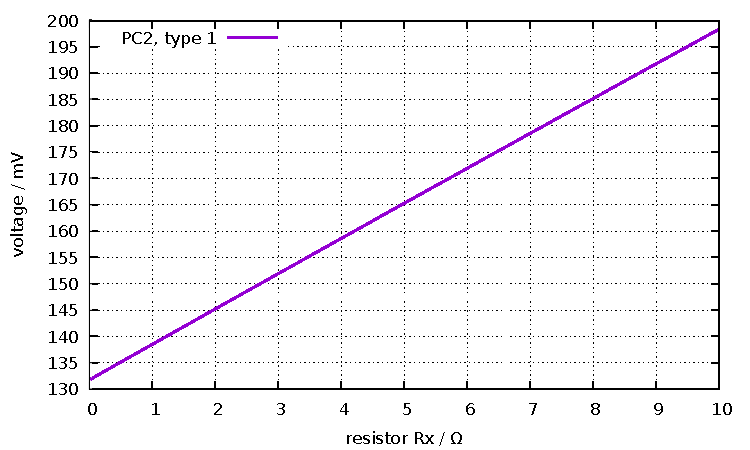
\includegraphics[width=1.\textwidth]{../GNU/RLvlow.pdf}
    \caption{Type 1 measurement}
    \label{fig:RLvlow}
  \end{subfigure}
  ~
  \begin{subfigure}[b]{.5\textwidth}
    \centering
    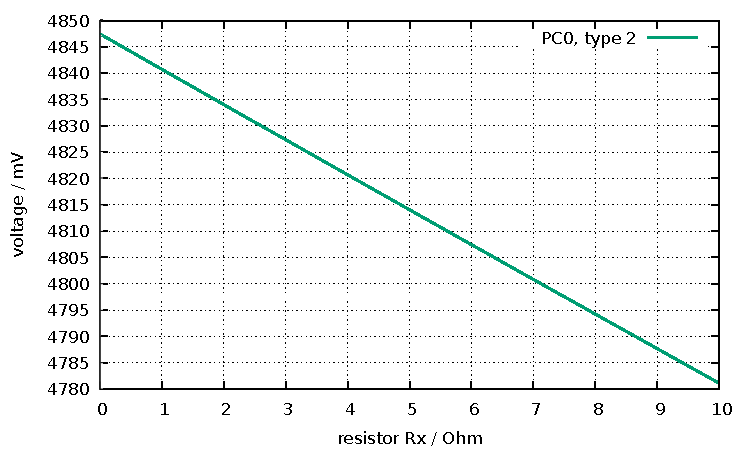
\includegraphics[width=1.\textwidth]{../GNU/RLvhigh.pdf}
    \caption{Type 2 measurement}
    \label{fig:RLvhigh}
  \end{subfigure}
  \caption{Cut-out of theoretical Voltage from \(0\Omega\) to \(10\Omega\)}
\end{figure}


\subsection{Resistor Measurement with 470 kOhm resistors}
The next figures~\ref{fig:RH1mes} and \ref{fig:RH2mes} shows the same measurement procedure for the
measurement with the precision \(470k\Omega\) resistors. Because the \(470k\Omega\) is very big in relation
to the port resistor values \(22\Omega\) and \(19\Omega\), the port resistor values are ignored for the computing
of the resistor value Rx.

For both measurement types with the \(470k\Omega\) resistors only one Voltage is measured, because the current
is so low, that no voltage difference at the internal port resistors of the ATmega can be measured (as expected).
The theoretical voltage gradient is shown in figure~\ref{fig:RHv} where the resistor values are again shown in logarithmic scale.
The theoretical gradient in this diagram ends at \(100M\Omega\), but the resulting value of the Tester is
limited to \(60M\Omega\), otherwise the Tester assumes that no resistor is connected.
The weighted average of both measurement types is taken as result with the same rules described for the measurements with the \(680\Omega\) resistors.
For all ATmega processors I had found, that the measured results with the \(470k\Omega\) resistors are more exactly,
if a constant offset of \(350\Omega\) will be added.
This offset can be adjusted with the RH\_OFFSET define in the config.h file.

\begin{figure}[H]
\centering
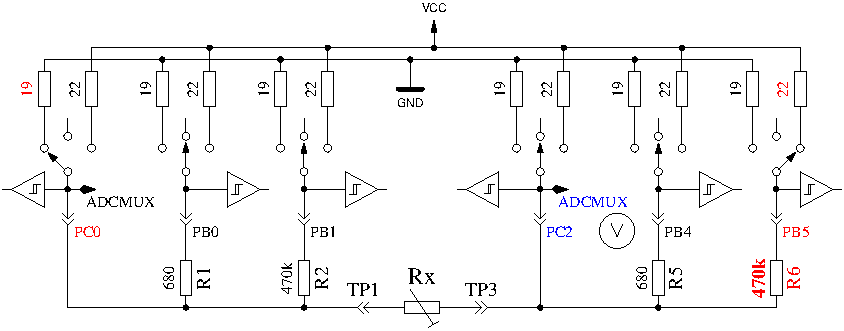
\includegraphics[width=.8\textwidth]{../FIG/ResistormessH1.pdf}
\caption{Measurement type 3 with \(470k\Omega\) }
\label{fig:RH1mes}
\end{figure}

\begin{figure}[H]
 \centering
 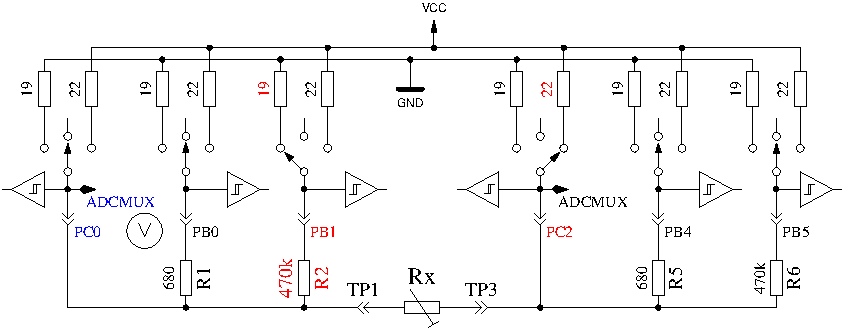
\includegraphics[width=.8\textwidth]{../FIG/ResistormessH2.pdf}
 \caption{Measurement type 4 with \(470k\Omega\) }
\label{fig:RH2mes}
\end{figure}

\begin{figure}[H]
\centering
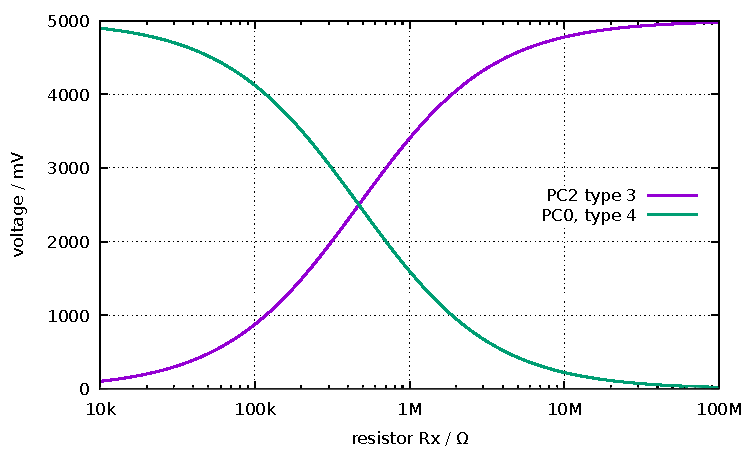
\includegraphics[width=.93\textwidth]{../GNU/RHv.pdf}
\caption{Voltages of type 3 and type 4 measurements with \(470k\Omega\) }
\label{fig:RHv}
\end{figure}

\subsection{Results of the resistor measurements}
Figure~\ref{fig:mega8res} shows the relative errors of the resistor measurements with three
ATmega8 microcontrollers. Additionally some results with the original software of Markus F.
with one ATmega8 are shown as ''Mega8orig'' in this figure.
More measurements results with ATmega8A and ATmega8L are shown in  figure~\ref{fig:mega8Ares} 
and \ref{fig:mega8Lres}.
Figure~\ref{fig:mega168res} shows the same measurements with a ATmega168 microcontroller.
Mega168 are the results without the AUTOSCALE\_ADC option, Mega168as are the same
measurements with the AUTOSCALE\_ADC option.
With the ATmega168 microcontroller it seems to be possible, that measurements of resistors
in the range from \(20\Omega\) to \(20M\Omega\) can be measured with a tolerance of \(\pm1\%\).
For Measurements below \(100\Omega\) you should keep in mind, that any measurement probe with
wire have a resistance too. It is better to connect the resistor directly to the terminal pins.
If this is not possible, subtract the resistance value of the shortened probe.
For example, if your Resistor have a printed value of \(30\Omega\), your tester shows a value of \(30.6\Omega\)
and the two probes shortened have a value of \(0.5\Omega\), then your resistor has been measured
with \(30.1\Omega\).
Below a resistance value of \(10\Omega\) one resolution step results to a error of more than \(1\%\)!

\begin{figure}[H]
\centering
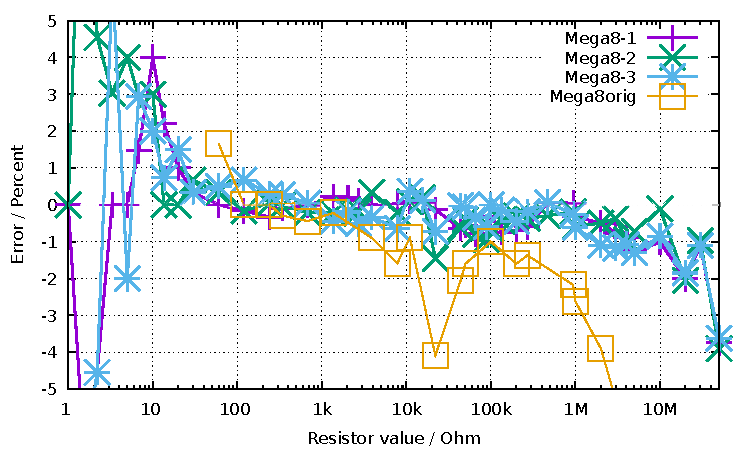
\includegraphics[width=.93\textwidth]{../GNU/Mega8res.pdf}
\caption{Relative error for resistor measurements with ATmega8 }
\label{fig:mega8res}
\end{figure}

\begin{figure}[H]
  \begin{subfigure}[b]{.5\textwidth}
    \centering
    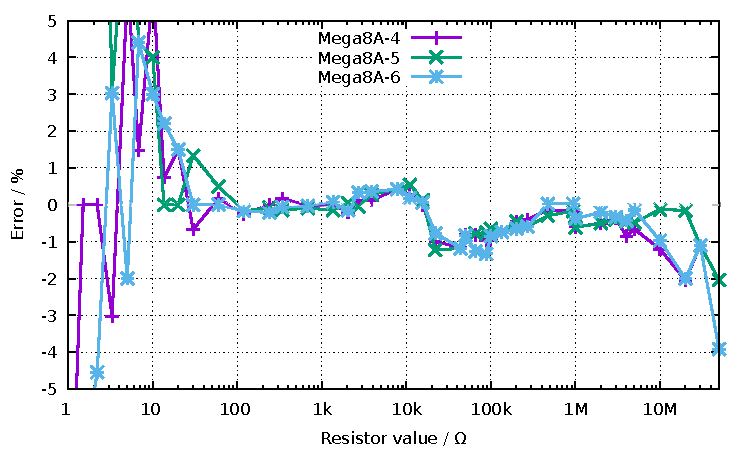
\includegraphics[width=1.\textwidth]{../GNU/Mega8Ares.pdf}
    \caption{with three ATmega8A}
    \label{fig:mega8Ares}
  \end{subfigure}
  ~
  \begin{subfigure}[b]{.5\textwidth}
    \centering
    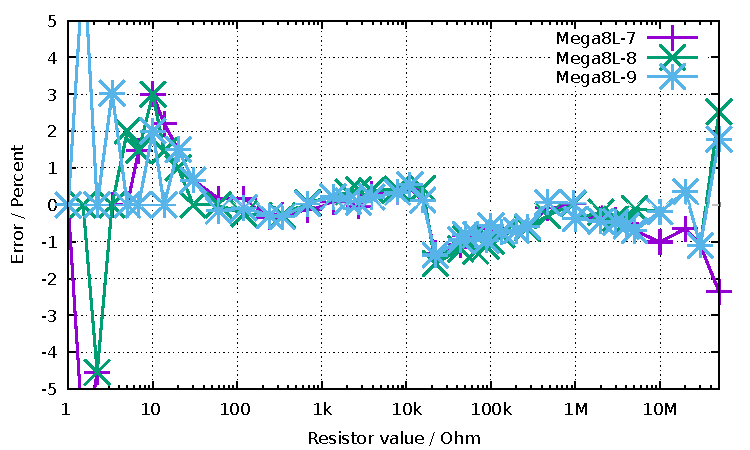
\includegraphics[width=1.\textwidth]{../GNU/Mega8Lres.pdf}
    \caption{with three ATmega8L}
    \label{fig:mega8Lres}
  \end{subfigure}
\caption{Relative error for resistor measurements}
\end{figure}


\begin{figure}[H]
\centering
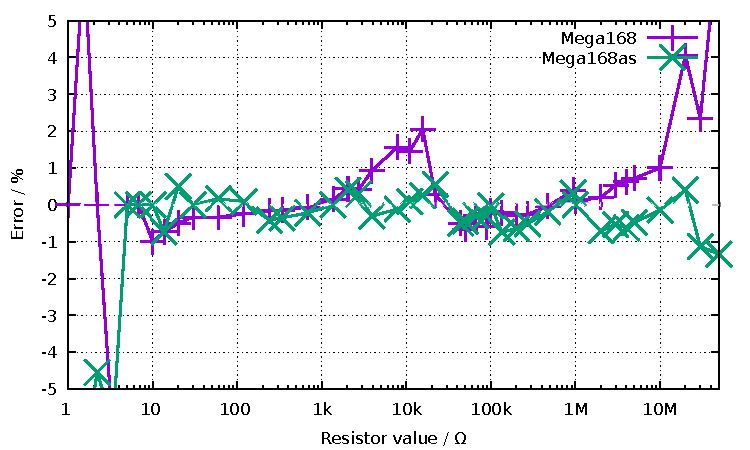
\includegraphics[width=.93\textwidth]{../GNU/Mega168res.pdf}
\caption{Relative error for resistor measurements with ATmega168 }
\label{fig:mega168res}
\end{figure}

The figure \ref{fig:m168res_all} shows the measurement errors of three ATmega168 processors before calibration as points, after the
calibration as line. The equivalent measurement errors of three ATmega168A prozessors are shown in figure \ref{fig:m168ares_all} and
the measurement errors of three ATmega168P prozessors are shown in figure \ref{fig:m168pres_all} .
The measurement errors of three ATmega328 prozessors are shown in figure \ref{fig:m328res_all} and \ref{fig:m328pres_all}.
After the automatic calibration the relative measurement errors of resistors between \(10\Omega~-~20 M\Omega\) 
usually are in the limit \(\pm1\%\). Only one measurement of a \(22k\Omega\) resistor with the ATmega328P-13 shows 
a higher error.
Before the calibration errors of some processors are found with \(\pm3\%\).
This will be caused by the AUTOSCALE\_ADC switching of the ADC reference.
The direct compare of a capacitor voltage below 1~V, once measured with the VCC reference and another once measured with 
the internal reference, can adjust this error.
With this measurement condition the voltage is measured with the same multiplexor channel and the internal bandgap reference
is connected to the AREF pin of the ATmega.
Unfortunately the direct measurement of the bandgap reference with the special multiplexor channel results to this offset,
which can be manually adjusted with the REF\_R\_KORR option or automatically with the AUTO\_CAL option of the selftest.
With the AUTO\_CAL option the REF\_R\_KORR value is a additional offset to the automatic find out value!

\begin{figure}[H]
  \begin{subfigure}[b]{.5\textwidth}
    \centering
    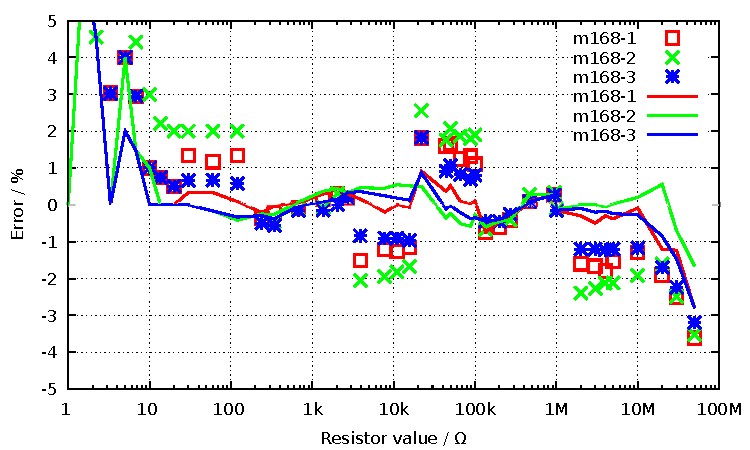
\includegraphics[width=1.\textwidth]{../GNU/m168res_all.pdf}
    \caption{with three ATmega168}
    \label{fig:m168res_all}
  \end{subfigure}
  ~
  \begin{subfigure}[b]{.5\textwidth}
    \centering
    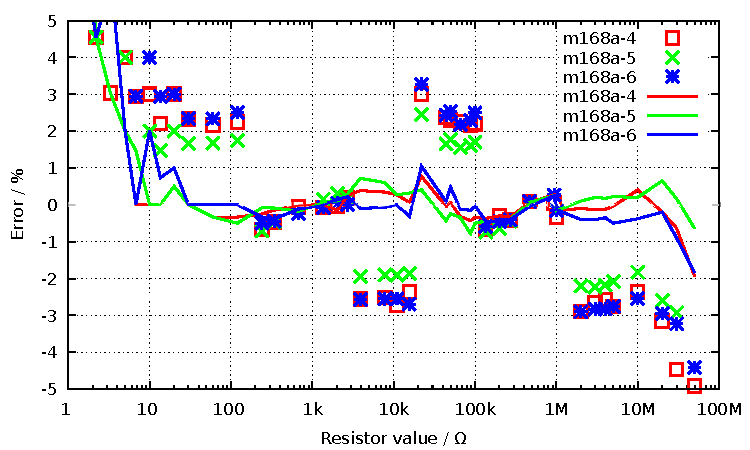
\includegraphics[width=1.\textwidth]{../GNU/m168ares_all.pdf}
    \caption{with three ATmega168A}
    \label{fig:m168ares_all}
  \end{subfigure}
\caption{Relativ error for resistor measurements}
\end{figure}

\begin{figure}[H]
\centering
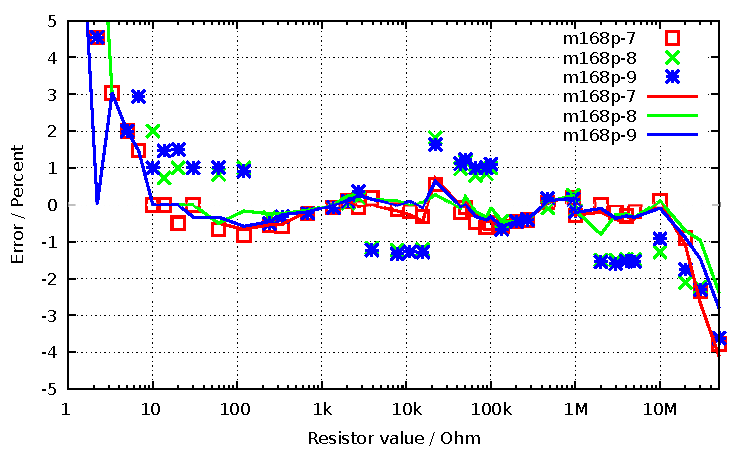
\includegraphics[width=.93\textwidth]{../GNU/m168pres_all.pdf}
\caption{Relativ error for resistor measurements with three ATmega168P }
\label{fig:m168pres_all}
\end{figure}

\begin{figure}[H]
  \begin{subfigure}[b]{.5\textwidth}
    \centering
    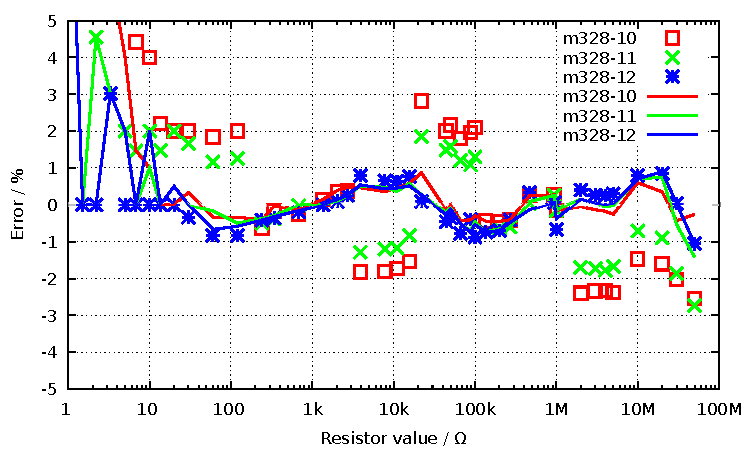
\includegraphics[width=1.\textwidth]{../GNU/m328res_all.pdf}
    \caption{with three ATmega328}
    \label{fig:m328res_all}
  \end{subfigure}
  ~
  \begin{subfigure}[b]{.5\textwidth}
    \centering
    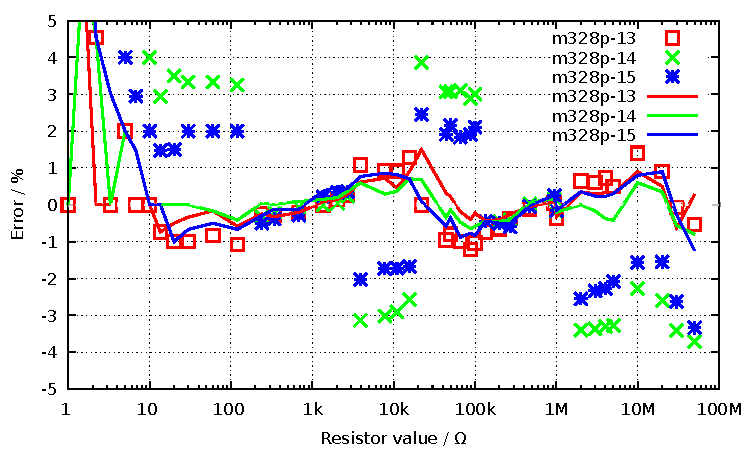
\includegraphics[width=1.\textwidth]{../GNU/m328pres_all.pdf}
    \caption{with three ATmega328P}
    \label{fig:m328pres_all}
  \end{subfigure}
\caption{Relativ error for resistor measurements}
\end{figure}

